\documentclass{article}
\linespread{0.7}
\usepackage[a4paper, margin=3mm, landscape]{geometry}
\usepackage{multicol}
\usepackage{xcolor}
\usepackage{enumitem}
\usepackage{amsmath}
\usepackage{amsfonts}
\usepackage{listings}
\usepackage{soul}
\usepackage{graphicx}

\pdfinfo{
    /Title (cs2103t.pdf)
    /Creator (TeX)
    /Producer (pdfTeX 1.40.0)
    /Author (Vincent Pang)
    /Subject (template)
    /Keywords (cheatsheet, pdf, cs2103t)
}

\graphicspath{ {./img/} }

\pagestyle{empty}
\setcounter{secnumdepth}{0}
\setlength{\columnseprule}{0.25pt}

% Redefine section commands to use less space
\makeatletter
\renewcommand{\section}{\@startsection{section}{1}{0mm}%
    {-1ex plus -.5ex minus -.2ex}%
    {0.5ex plus .2ex}%x
{\normalfont\large\bfseries}}
\renewcommand{\subsection}{\@startsection{subsection}{2}{0mm}%
    {-1explus -.5ex minus -.2ex}%
    {0.5ex plus .2ex}%
{\normalfont\normalsize\bfseries}}
\renewcommand{\subsubsection}{\@startsection{subsubsection}{3}{0mm}%
    {-1ex plus -.5ex minus -.2ex}%
    {1ex plus .2ex}%
{\normalfont\small\bfseries}}%
\makeatother

% Adjust spacing for all itemize/enumerate
\setlength{\leftmargini}{0.5cm}
\setlength{\leftmarginii}{0.5cm}
\setlist[itemize,1]{leftmargin=2mm,labelindent=1mm,labelsep=1mm}
\setlist[itemize,2]{leftmargin=2mm,labelindent=1mm,labelsep=1mm}

% Font
\renewcommand{\familydefault}{\sfdefault}

% Define colors for math formulas
\definecolor{myblue}{cmyk}{1,.72,0,.38}
\everymath\expandafter{\the\everymath \color{myblue}}

% Custom command for keywords
\definecolor{highlight}{RGB}{251,243,218}
\newcommand{\keyword}[2][]{\sethlcolor{highlight}\hl{\textbf{#2}} #1 - }
\newcommand{\ilkeyword}[1]{\sethlcolor{highlight}\hl{\textbf{#1}}}

% Define colors and style for code
\definecolor{codegreen}{rgb}{0,0.6,0}
\definecolor{codegray}{rgb}{0.5,0.5,0.5}
\definecolor{codered}{HTML}{CC241D}
\definecolor{backcolor}{rgb}{0.95,0.95,0.95}
\lstdefinestyle{codestyle}{
    backgroundcolor = \color{backcolor},
    commentstyle = \color{codegray},
    keywordstyle = \color{codered},
    stringstyle = \color{codegreen},
    basicstyle = \ttfamily,
    breakatwhitespace = false,
    showstringspaces = false,
    breaklines = true,
    showtabs = false,
    tabsize = 2
}
\lstset{style = codestyle}

% -----------------------------------------------------------------------
\begin{document}
\begin{multicols*}{4}
\footnotesize

% Title box
\begin{center}
    \fbox{
        \parbox{0.8\linewidth}{
            \centering \textcolor{black}{
                {\Large\textbf{CS2103t}} \\
                \normalsize{Software Engineering 22/23s2 }} \\
                {\footnotesize \textcolor{gray}{github.com/securespider}}
        }
    }
\end{center}
{\Large \textbf{PE}}\\
\rule{6cm}{0.4pt}

\subsection{Bug reporting format}
\begin{itemize}
	\item Descriptive title with appropriate severity/type
	\item Steps to reproduce, expected, actual and screenshots
\end{itemize}
\section{UG}
\begin{itemize}
	\item Navigation does not work
\end{itemize}
\subsection{Visuals}
\begin{itemize}
	\item Not enough/unnecessarily repetitive pictures or improperly sized
	\item Visuals not integrated with the explanation
\end{itemize}
\subsection{Content}
\begin{itemize}
	\item Not enough/too many examples (input/outputs)
	\item Target user/value proposition not specified clearly
	\begin{itemize}
		\item Concise statement that explains to users how they benefit
	\end{itemize}
	\item Feature is not named appropriately or doesnt make sense
	\item Feature is not explained well for new users
	\item Info not the same as the application (error message different)
	\item Messy, improperly formatted, repetitive
\end{itemize}
\section{Product}
\subsection{Functionality Flaw}
\begin{itemize}
	\item Case sensitivity
	\item Error message does not match error
	\item Writing incorrect string types (age - five instead of 5)
	\item Giving values outside of boundary values (age - 999/0/-1)
	\item Long names/description/taglist/address
	\item try different date time formats/ dates that do not exist (leapyears)
	\item Are special characters legal?
	\item Test complicated features like undo and redo
	\item Giving duplicate objects/values
	\item Incorrect formats (age - 0001 != 1)
	\item Does not save correctly after closing and reopening
	\item How does product work if json file deleted mid-operation
\end{itemize}
\subsection{Feature Flaw}
\begin{itemize}
	\item Does not solve stated problem of intended user
	\item Features not well optimized for fast typist or target users
	\item Feature does not fit well with the product
\end{itemize}
\section{DG}
\subsection{General}
\subsubsection{Image}
\begin{itemize}
	\item Text in image not matching size of main text
	\item Image is not put close to where it is being described
	\item Lower level details of multiple components there without purpose
\end{itemize}
\subsection{Sequence Diagram}
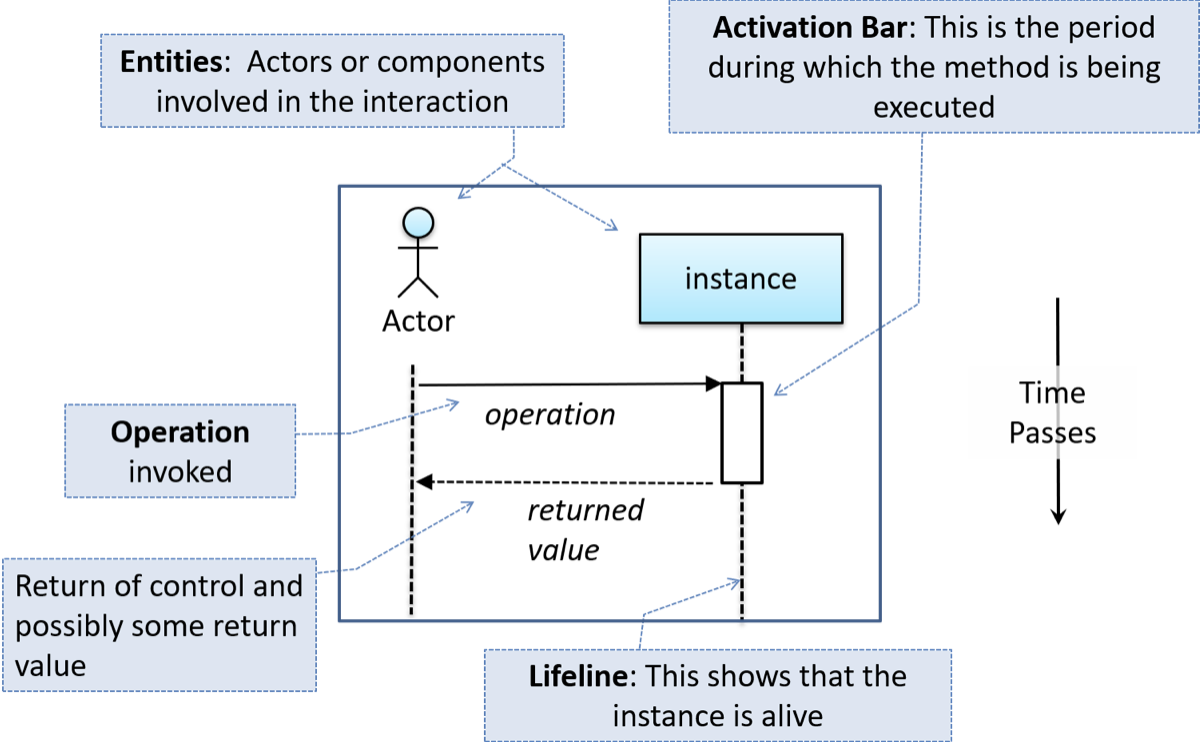
\includegraphics[scale=0.3]{sequence-diagram-basic}
\subsubsection{General}
\begin{itemize}
	\item Stay at the highest level of abstraction instead of the interactions that happen inside each component
	\item Use visual representation
	\begin{itemize}
		\item Associations and navigabilities using lines and arrows connecting classes instead of variables within classes
	\end{itemize}
\end{itemize}
\subsubsection{Arrows}
\begin{itemize}
	\item Must return control to caller
	\item Arrows representing method calls should be solid arrows whereas return should be dashed
	\item Return arrows are optional if it does not result in ambiguities or loss of relevant information
\end{itemize}
\subsubsection{Activation bar}
\begin{itemize}
	\item Activation bar of method cannot start before method call arrives and method cannot remain active after method has returned
	\begin{itemize}
		\item Arrow must start/end at the top/bottom tip of the activation bar
	\end{itemize}
	\item Activation bar should remain unbroken from point method is called until return
	\item These are optional
\end{itemize}
\subsubsection{Entities}
\begin{itemize}
	\item Entities should be in this format `instanceName:Class`
	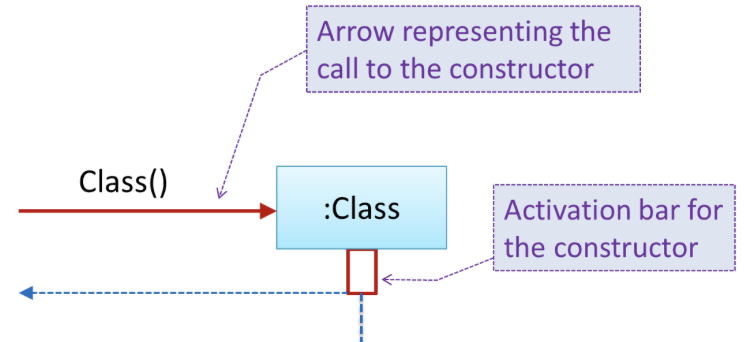
\includegraphics[scale=0.3]{sequence-diagram-obj-creation}
	\item X at the end of the lifeline of an object to show its deletion
	\item Method calls to static that are received by the class itself should have a $<<class>>$ at the top
\end{itemize}
\subsubsection{Paths}
\begin{itemize}
	\item Note that the boxes are not rectangles
\end{itemize}
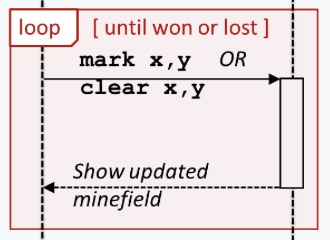
\includegraphics[scale=0.33]{sequence-diagram-loop}
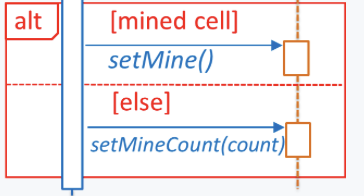
\includegraphics[scale=0.33]{sequence-diagram-alt}
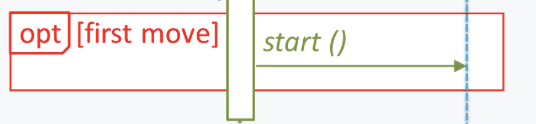
\includegraphics[scale=0.3]{sequence-diagram-opt}

\subsection{Activity Diagram}
\begin{itemize}
	\item Consist of start, action, flow/edge
\end{itemize}
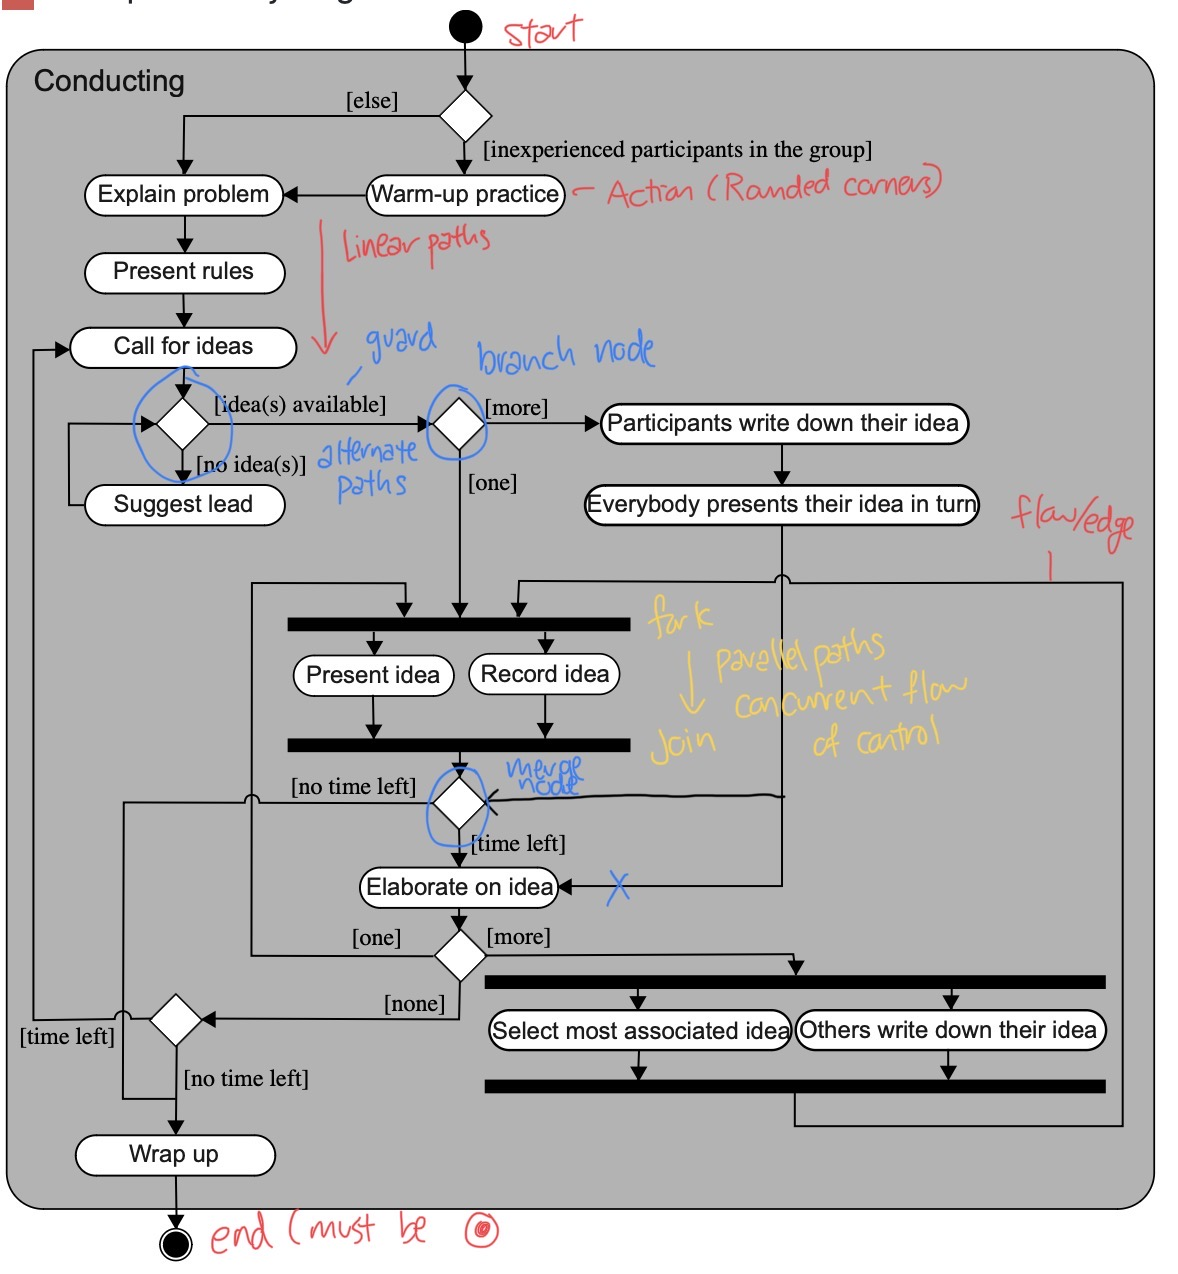
\includegraphics[scale=0.17]{activity-diagram-basic}
\subsubsection{Alternate paths}
\begin{itemize}
	\item Branch node shows start of alternate path with guard conditions
	\begin{itemize}
		\item \keyword{guard}{Boolean condition has to be true for execution to take the path}
	\end{itemize}
	\item Merge node and else conditions can be omited 
	\item Arrows \textbf{MUST} start from the corner
\end{itemize}
\subsubsection{Parallel path}
\begin{itemize}
	\item Execution along all parallel path \textbf{MUST} be complete before execution on outgoing path of join
\end{itemize}
\subsubsection{Rakes}
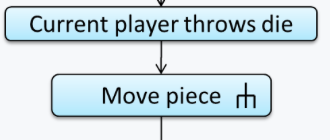
\includegraphics[scale=0.5]{activity-diagram-rake}
\begin{itemize}
	\item Indicate that a part of the activity is given as a separate diagram
\end{itemize}
\subsubsection{Swim lanes}
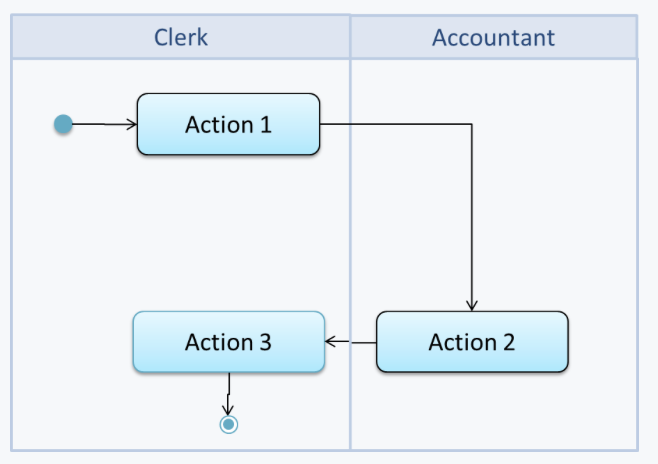
\includegraphics[scale=0.4]{activity-diagram-swimlane}
\begin{itemize}
	\item Partition activity diagram to show who is doing which action
\end{itemize}


\subsection{Class Diagram}
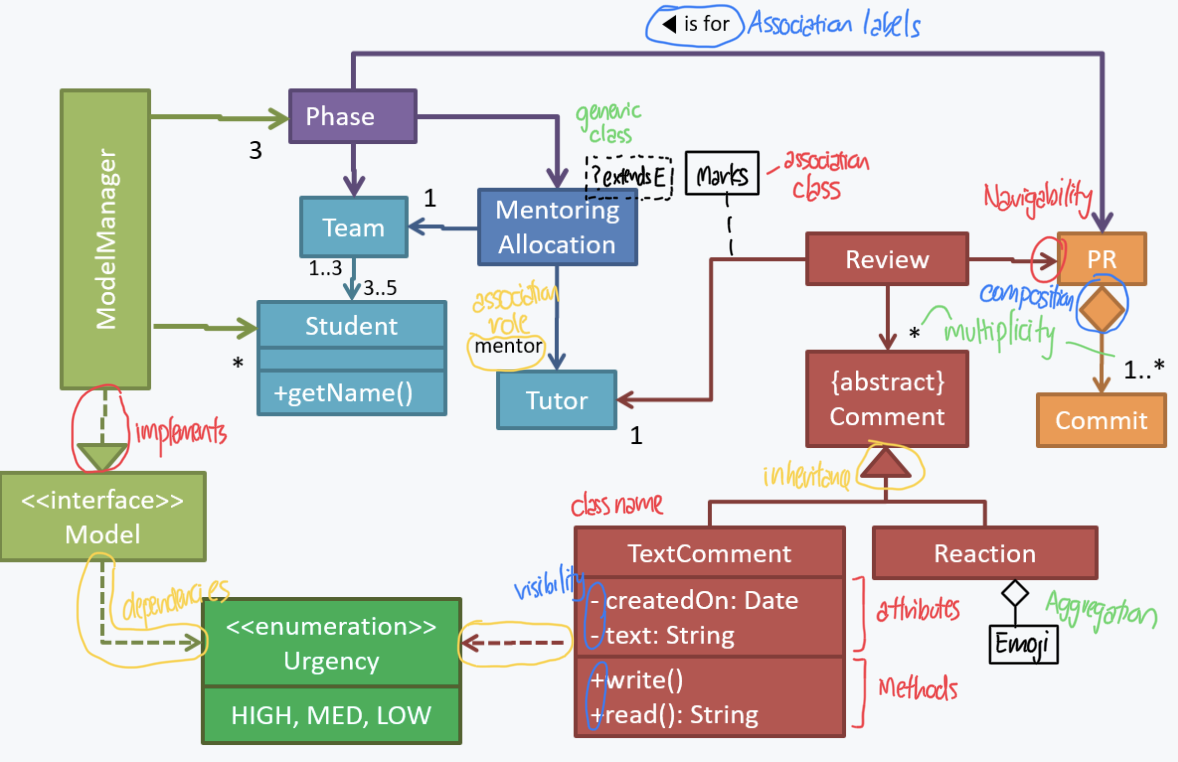
\includegraphics[scale=0.33]{class-diagram}
\subsubsection{Class representation}
\begin{itemize}
	\item Operations and attributes compartment can be omitted if not important
	\item Underlines denote class-level attributes and methods
\end{itemize}
\subsubsection{Visibility}
\begin{description}
	\item[+]{Public}
	\item[-]{Private}
	\item[\#]{Protected}
	\item[\~]{Package private}
\end{description}
\subsubsection{Associations}
\begin{itemize}
	\item Solid line that can have additional decorations like labels, roles, multiplicity and navigability
	\item Multiplicity (eg. m..n - between m and n inclusive, n - exactly n, * - 0 or more objects)
	\begin{itemize}
		\item If class A has multiplicity 2, means 2 objects of A associated to 1 object of other class
	\end{itemize}
	\item Navigability - There is a reference from one class to another (can be unidirectional or bidirectional)
\end{itemize}
\subsubsection{Composition vs Aggregation}
\begin{itemize}
	\item Composition represents strong whole-part relationship 
	\begin{itemize}
		\item If whole is destroyed, parts are destroyed too (eg. Person = whole, name = part)
		\item Commonly used when parts of a big class carved into smaller class for better management
		\item Solid diamond
	\end{itemize}
	\item Aggregation represents container-contained relationship
	\begin{itemize}
		\item Containee object can exist even after container object is deleted (eg. Person in a team)
		\item Hollow diamond
	\end{itemize}
\end{itemize}
\subsubsection{Dependencies vs association}
\begin{description}
	\item[Association]{Object keeping reference of another}
	\item[Dependency]{Class accessing some method/value of another but no association}
\end{description}
\subsubsection{Inheritance}
\begin{itemize}
	\item Abstract classes/methods should either be italicised or with `$\{abstract\}$` keyword
\end{itemize}
\subsubsection{Association Classes}
\begin{itemize}
	\item Represents additional information about association
	\item Should be dotted from the association btw 2 classes
\end{itemize}

\subsection{Object Diagram}
\subsubsection{Objects}
\begin{itemize}
	\item Class name and object name (optional) must be underlined in the format `objectName:ClassName`
	\item Should not include methods, only attributes that are relevant to the task
\end{itemize}

\subsection{Non-functional requirements}
\begin{itemize}
	\item Specify the constraints under which the system is developed and operated
\end{itemize}
\subsubsection{Example requirements}
\begin{description}
	\item[Data]{Size, volatility, persistency (shouldnt be more than 20MB, no crashes, respond within 2s)}
	\item[Environment]{Technical environment which the system would operate in or need to be compatible in (work on 32-bit systems with java installed)}
\end{description}
\subsubsection{Characteristics}
\begin{itemize}
	\item Unambiguous, testable, clear, feasible, atomic (indivisible), necessary, \textbf{implementation-free}
	\item Consistent, non-redundant, complete
\end{itemize}

\subsection{User Stories}
\begin{itemize}
	\item Short simple descriptions of a feature told from perspective of person who wants the capability
	\item Must be in the format `As a \{user type/role\} I can \{function\} so that \{benefit\}`
	\begin{itemize}
		\item Benefit can be omitted if obvious
	\end{itemize}
	\item User story should not include any implementation details
\end{itemize}
\subsection{Use cases}
\begin{itemize}
	\item Interaction between the user and system for specific functionality of system
	\item Should only describe externally visible behaviour not internal details of a system
	\begin{itemize}
		\item This is wrong: LMS \textit{saves file into cache} and indicate success
	\end{itemize}
	\item Step should give the intention of the actor instead of the mechanics
	\begin{itemize}
		\item UI details should be omitted to give UI designer flexibility in implementation
	\end{itemize}
	\item Can include other use case which \textbf{MUST BE underlined} (inclusions)
\end{itemize}
\subsubsection{Main Success Scenario (MSS)}
\begin{itemize}
	\item Most straightforward interaction for a given use case, assuming nothing goes wrong
	\item Should be self-contained (complete usage scenario)
\end{itemize}
\subsubsection{Extensions}
\begin{itemize}
	\item Add on to the MSS that describes exceptional/alternative flow of events
	\item Extensions should be numerically marked based on when the event may happen
	\begin{itemize}
		\item Extensions marked 3a. happens just after step 3 of MSS (3a1, 3a2...)
		\item Extensions marked *a happens at any step (*a1, *a2...)
		\item Subsequent extensions will be 3b, 4a or *b...
	\end{itemize}
\end{itemize}
\subsubsection{Format}
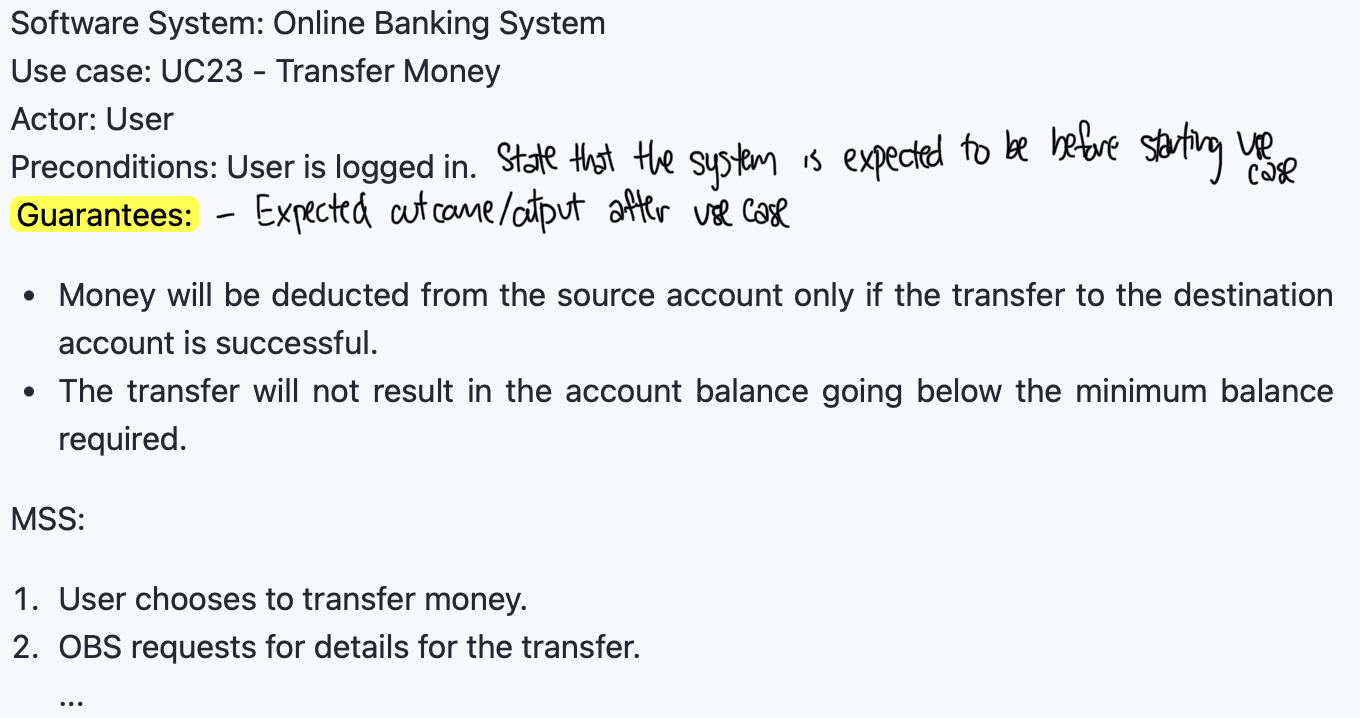
\includegraphics[scale=0.28]{use-case}

\end{multicols*}
\end{document}
